\chapter{Marco Teórico}

\section{Internet de las Cosas}

La internet de las cosas es un sistema de dispositivos de computación interrelacionados, máquinas mecánicas y digitales, objetos, animales o personas que tienen identificadores únicos y la capacidad de transferir datos a través de una red, sin requerir de interacciones humano a humano o humano a computadora. \\

IoT ha evolucionado desde la convergencia de tecnologías inalámbricas, sistemas micro-electromecánicos, microservicios e Internet. La convergencia ha ayudado a derribar las paredes de silos entre la tecnología operativa y la tecnología de la información, permitiendo que los datos no estructurados generados por máquinas sean analizados para obtener información que impulse mejoras. \cite{TechT2017}\\

Kevin Ashton, cofundador y director ejecutivo del Auto-ID Center de MIT, mencionó por primera vez la internet de las cosas en una presentación que hizo a Procter \& Gamble en 1999. He aquí cómo Ashton explica el potencial del internet de las cosas:

``Las computadoras de hoy –y, por lo tanto, la internet– dependen casi totalmente de los seres humanos para obtener información. Casi todos los aproximadamente 50 petabytes (un petabyte son 1.024 terabytes) de datos disponibles en internet fueron capturados y creados por seres humanos escribiendo, presionando un botón de grabación, tomando una imagen digital o escaneando un código de barras. \\

El problema es que la gente tiene tiempo, atención y precisión limitados, lo que significa que no son muy buenos para capturar datos sobre cosas en el mundo real. Si tuviéramos computadoras que supieran todo lo que hay que saber acerca de las cosas –utilizando datos que recopilaron sin ninguna ayuda de nosotros– podríamos rastrear y contar todo, y reducir en gran medida los desechos, las pérdidas y el costo. Sabríamos cuándo necesitamos reemplazar, reparar o recordar cosas, y si eran frescas o ya pasadas”. \cite{Asthon2009}

\subsection{Plataforma Heroku}

``Heroku es una plataforma en la nube basada en un sistema gestionado por contenedores, con servicios de datos integrados y un potente ecosistema para desarrollar y ejecutar aplicaciones modernas. La experiencia de los desarrolladores de Heroku es un enfoque centrado en aplicaciones para la entrega de software, integrado con las herramientas y flujos de trabajo de desarrollador más populares de la actualidad'' \cite{Hero}.


\subsection{Framework Laravel}

``Laravel es un framework de aplicaciones web con una sintaxis expresiva y elegante. Laravel intenta aliviar el dolor del desarrollo al facilitar las tareas comunes que se utilizan en la mayoría de los proyectos web, como la autenticación, el enrutamiento, las sesiones y el almacenamiento en caché.\\

Laravel tiene como objetivo hacer que el proceso de desarrollo sea agradable para el desarrollador sin sacrificar la funcionalidad de la aplicación. Con este fin, se ha intentado combinar lo mejor de lo que hemos visto en otros marcos web, incluidos los marcos implementados en otros lenguajes, como Ruby on Rails, ASP.NET MVC y Sinatra.\\

Laravel es accesible, pero potente, y proporciona potentes herramientas necesarias para aplicaciones grandes y robustas. Una magnífica inversión de contenedores de control, un sistema de migración expresivo y un soporte de prueba de unidades estrechamente integrado le brindan las herramientas que necesita para construir cualquier aplicación'' \cite{Lara}.

\subsection{HTTP}

El protocolo de transferencia de hipertexto (HTTP) es un protocolo de la capa de aplicación en el modelo OSI, usado para transmitir documentos hipermedia como HTML. Diseñado con el propósito de la comunicación entre navegadores y servidores web, no obstante, puede operar con otros propósitos. HTTP sigue un modelo clásico de cliente-servidor, con un cliente que abre una conexión y realiza una petición a la espera de respuesta. HTTP es un protocolo sin estado, significa que el servidor no conserva ningún dato entre dos solicitudes. Para realizar las peticiones, este protocolo cuenta con diferentes metodos \cite{HTTP}.

\paragraph{Métodos de solicitud HTTP:}

HTTP define un conjunto de métodos de solicitudes para indicar la acción deseada que se realizará a un recurso determinado. Aunque pueden ser sustantivos, estos métodos algunas veces se denominan verbos HTTP. Cada uno de ellos implementa una semántica diferente, pero algunas características comunes son compartidas por un grupo de ellos \cite{HTTPM}.\\

\begin{itemize}
	\item GET: este método solicita una representación del recurso especificado. Las peticiones que lo usan, solo deben regresar datos.
	\item HEAD: este método solicita una respuesta igual a una peticion GET, pero sin el cuerpo de la respuesta.
	\item POST: se usa para enviar una entidad al recurso especificado, causando a menudo un cambio en el estado o efectos secundarios en el servidor.
	\item PUT: reemplaza todas las representaciones actuales del recurso destino con la la petición de carga útil.
	\item DELETE: esta petición elimina el recurso especificado.
	\item CONNECT: establece un túnel para el servidor identificado por el recurso de destino.
	\item OPTIONS: se usa para describir las opciones de la comunicación para el recurso destino.
	\item TRACE: realiza una prueba de mensaje loop-back a lo largo de la ruta del recurso de destino. 
	\item PATCH: se usa para realizar modificaciones parciales a un recurso.
\end{itemize}

\subsection{JSON}

``JSON (JavaScript Object Notation - Notación de Objetos de JavaScript) es un formato ligero de intercambio de datos. Leerlo y escribirlo es cómodo para los humanos, al igual que para las máquinas resulta simple interpretarlo y generarlo. Está basado en un subconjunto del Lenguaje de Programación JavaScript, Standard ECMA-262 3rd Edition - Diciembre 1999. JSON es un formato de texto que es completamente independiente del lenguaje pero utiliza convenciones que son ampliamente conocidos por los programadores de la familia de lenguajes C, incluyendo C, C++, C\#, Java, JavaScript, Perl, Python, y muchos otros. Estas propiedades hacen que JSON sea un lenguaje ideal para el intercambio de datos'' \cite{JSON}.\\

JSON está constituído por dos estructuras:

\begin{itemize}
	\item Una colección de pares de nombre/valor. En varios lenguajes esto es conocido como un objeto, registro, estructura, diccionario, tabla hash, lista de claves o un arreglo asociativo.
	
	\item Una lista ordenada de valores. En la mayoría de los lenguajes, esto se implementa como arreglos, vectores, listas o secuencias.
\end{itemize}

Estas son estructuras universales; virtualmente todos los lenguajes de programación las soportan de una forma u otra. Es razonable que un formato de intercambio de datos que es independiente del lenguaje de programación se base en estas estructuras \cite{JSON}.

\subsection{Base de Datos}

``Se define una base de datos como una serie de datos organizados y relacionados entre sí, los cuales son recolectados y explotados por los sistemas de información de una empresa o negocio en particular.

Cada base de datos se compone de una o más tablas que guarda un conjunto de datos. Cada tabla tiene una o más columnas y filas. Las columnas guardan una parte de la información sobre cada elemento que queramos guardar en la tabla, cada fila de la tabla conforma un registro'' \cite{DB}. \\

Para la gestión de datos es muy común encontrar las funciones básicas de crear, leer, actualizar y borrar (CRUD), con la finalidad de que el usuario final pueda acceder a estos sin necesidad de realizar peticiones directamente a la base de datos, sino en una interfaz gráfica (GUI).

\section{Smart House}

El concepto de Smart House implica tres características básicas. En primer lugar, el monitoreo a través de redes de sensores para obtener información sobre la casa y sus residentes. En segundo lugar, los mecanismos que controlan el uso de la comunicación entre dispositivos con el fin de permitir la automatización y el acceso remoto. Por último, las interfaces de usuario, como los teléfonos inteligentes y las computadoras que permiten a los usuarios especificar las preferencias, así como presentar información a las personas acerca de estas. \\

Smart House es un entorno que tiene sistemas sofisticados a través de los cuales se pueden controlar algunos de los objetos de la casa, como luces, puertas, ventanas, además puede racionalizar el consumo de energía, entre otras funciones mediante el uso de sensores. Básicamente, uno de los beneficios más importantes del uso de la tecnología en las casas, es la prestación de servicios a las personas.\cite{Howedi2016} 

\section{Hardware}

\subsection{ESP-WROOM-32}

Es un potente módulo MCU Wi-Fi + BT + BLE que se dirige a una amplia variedad de aplicaciones, desde redes de sensores de baja potencia hasta las tareas más exigentes, como codificación de voz, transmisión de música y decodificación de MP3, además de su reducido tamaño, según se observa en la Figura \ref{fig:esp32-wroom-s32-00}.\\

En el núcleo de este módulo está el chip ESP32-D0WDQ6. El chip integrado se encuentra diseñado para ser escalable y adaptable. Hay dos núcleos de CPU que se pueden controlar individualmente, y la frecuencia del reloj es ajustable de 80 MHz a 240 MHz. El usuario también puede apagar la CPU y utilizar el coprocesador de baja potencia para monitorear constantemente los periféricos en busca de cambios o cruces de umbrales. ESP32 integra un amplio conjunto de periféricos, que van desde sensores táctiles capacitivos, sensores Hall, interfaz de tarjeta SD, Ethernet, SPI de alta velocidad, UART, I2S e I2C.\\

La integración de Bluetooth, Bluetooth LE y Wi-Fi garantiza que se pueda orientar una amplia gama de aplicaciones, el uso de Wi-Fi permite un gran alcance físico y conexión directa a Internet a través de este, mientras usa Bluetooth, le permite al usuario conectarse convenientemente al teléfono o transmitir balizas de baja energía para su detección. La corriente de reposo del chip ESP32 es inferior a 5 $\mu$A, lo que lo hace adecuado para aplicaciones de electrónica con batería y portátiles. ESP32 admite una velocidad de datos de hasta 150 Mbps y una potencia de salida de 20.5 dBm en la antena con el objetivo de garantizar el rango físico más amplio.\\

El sistema operativo elegido para ESP32 es freeRTOS con LwIP; TLS 1.2 con aceleración de hardware está integrado también, además se admite la actualización segura (cifrada) a través del aire (OTA), de modo que los desarrolladores puedan actualizar continuamente sus productos incluso después de su lanzamiento.\cite{EW32}

\begin{figure}[H]
	\centering
	\caption[ESP WROOM 32.]{ESP WROOM 32. Tomado de: \cite{ESPIMG}}
	\label{fig:esp32-wroom-s32-00}
	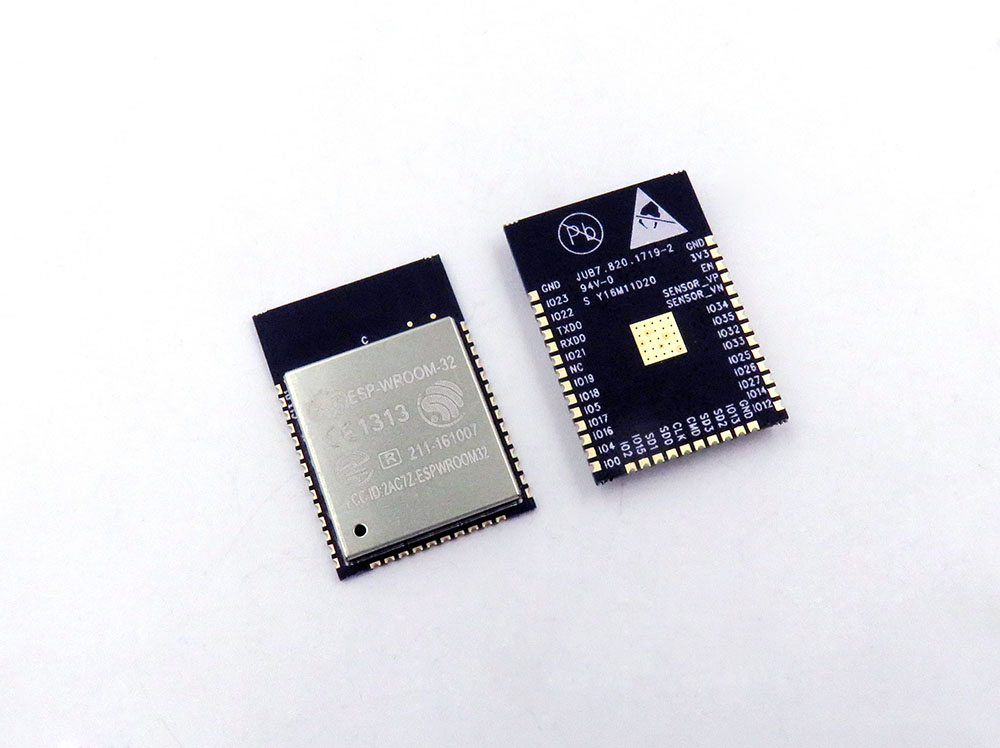
\includegraphics{Imagenes/esp32-wroom-s32-00}
\end{figure}

\subsection{Corriente Alterna (AC)}

``Es un tipo de corriente eléctrica, en la que la dirección del flujo de electrones va y viene a intervalos regulares o en ciclos. La corriente que fluye por las líneas eléctricas y la electricidad disponible normalmente en las casas procedente de los enchufes de la pared es corriente alterna. La corriente estándar utilizada en los EE.UU. es de 60 ciclos por segundo (es decir, una frecuencia de 60 Hz); en Europa y en la mayor parte del mundo es de 50 ciclos por segundo (es decir, una frecuencia de 50 Hz.)''. \cite{Cor}

\subsection{Corriente Directa (DC)}

``Es la corriente eléctrica que fluye de forma constante en una dirección, como la que fluye en una linterna o en cualquier otro aparato con baterías es corriente continua.

Una de las ventajas de la corriente alterna es su relativamente económico cambio de voltaje. Además, la pérdida inevitable de energía al transportar la corriente a largas distancias es mucho menor que con la corriente continua''. \cite{Cor}

\subsection{Control de potencia AC por ángulo de fase}

``Los SCR y los TRIAC, permiten aplicar una técnica muy conveniente y eficaz para controlar el voltaje promedio y por lo tanto la potencia aplicada a una carga, cambiando el ángulo de fase con el cual la fuente de voltaje se aplica a ésta. Esta técnica de control de voltaje es muy usada en las aplicaciones de regulación de motores, iluminación y temperatura, por ser el voltaje la variable principal en estos tres procesos''.\cite{CEKIT}\\

``Para entender como se controla el ángulo de fase, por medio de un TRIAC conectado en serie con la carga, se puede asumir que el TRIAC se comporta idealmente como un interruptor controlador por la corriente de compuerta Ig que se cierra o se abre ante su presencia o ausencia. Observando la Figura \ref{fig:triacgraph} puede verse el control de una onda seno de tensión con un período con un período de 360 grados; en la parte (a) de la figura se muestra la tensión a través del TRIAC, mientras que en la parte (b) se ve la tensión sobre la carga; allí puede verse que el TRIAC se comporta como un circuito abierto durante los primero 45 grados de cada semiciclo, y todo el voltaje cae en sus terminales eliminando el flujo de corriente por la carga. La porción del semiciclo durante la cual se presenta esta situación se conoce como ángulo de disparo''\cite{CEKIT}.\\

``Una vez el TRIAC es disparado a través de su terminal de compuerta (G), éste se engancha y se comporta como un interruptor cerrado, permitiendo que todo el voltaje se aplique a la carga durante los 135 grados restantes de cada semiciclo. La porción del semiciclo durante la cual el TRIAC conduce se denomina ángulo de conducción''\cite{CEKIT}.

\begin{figure}[H]
	\centering
	\caption[Representación gráfica del ángulo de disparo y de conducción del TRIAC y de la carga.]{Representación gráfica del ángulo de disparo y de conducción del TRIAC y de la carga. Tomado de: \cite{CEKIT}.}
	\label{fig:triacgraph}
	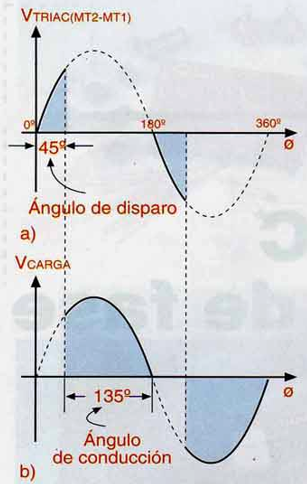
\includegraphics[width=0.3\linewidth]{Imagenes/TRIAC_graph}
\end{figure}

\subsection{Control de Cargas DC}

Los transistores como switch permiten controlar las cargas de corriente continua con ayuda de una señal PWM que los activa o desactiva. Las cargas de corriente continuas típicas como los motores y LED's, a parte de poder funcionar en dos estados, encendido y apagado, pueden se controladas mediante la modulación por ancho de pulso (PWM), ya que al variar el ancho de pulso de la señal eléctrica se varia la cantidad de energía entregada a la carga, por ejemplo, si es un LED el cambio se refleja en su intensidad lumínica y si es un motor DC cambia su velocidad de giro \cite{PWM}. Este control se produce gracias a que en esta modulación se modifica su ciclo útil, cambiando el tiempo en que la señal eléctrica se encuentra en alto durante un periodo, por lo tanto si el ciclo útil es del 10\% el poder entregado es poco, en comparación, con un ciclo útil del 50\% o 100\% conforme se observa en la Figura \ref{fig:pwm-duty-800x396}.

\begin{figure}[H]
	\centering
	\caption[Ciclo Útil PWM.]{Ciclo Útil PWM. [Imagen Propia] }
	\label{fig:pwm-duty-800x396}
	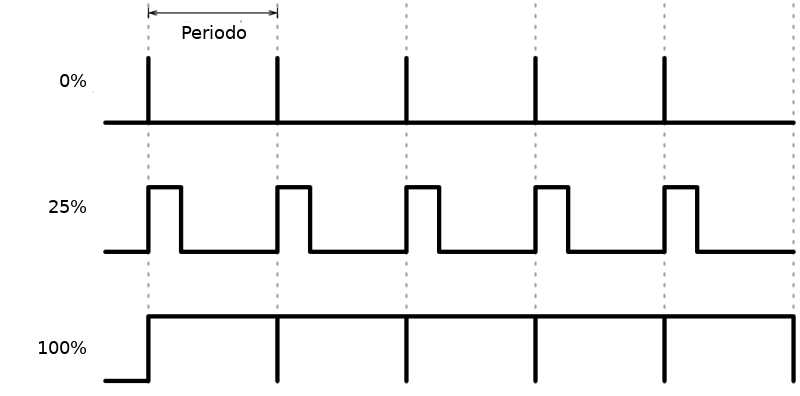
\includegraphics[width=0.5\linewidth]{Imagenes/pwm}
\end{figure}


\subsection{I2C}

``I2C es un puerto y protocolo de comunicación serial, define la trama de datos y las conexiones físicas para transferir bits entre 2 dispositivos digitales. El puerto incluye dos cables de comunicación, SDA y SCL. Además el protocolo permite conectar hasta 127 dispositivos esclavos con esas dos líneas, con hasta velocidades de 100, 400 y 1000 kbits/s. También es conocido como IIC ó TWI – Two Wire Interface'' \cite{I2C}.

\subsection{Sensores}\label{sec:sensors}

\subsubsection{Módulo GY-30}

``Sensor GY-30 BH1750FVI. Es un sensor digital de intensidad de luz ambiente, tiene un conversor ADC de 16bits interno y comunicación por I2C como se observa en la Figura \ref{fig:gy-30}. Esta es una versión mejorada del típico sensor de luz a base de un LDR, el cual simplemente entrega un valor analógico. Compatible con Arduino, PIC, etc. \\

El módulo BH1750 es un sensor de luz, que a diferencia del LDR es digital y nos entrega valores de medición en Lux ( lumen /m$^2$ ) que es una  unidad de medida estándar para el nivel de iluminación (iluminancia). Tiene alta precisión y un rango ente 1 – 65535 lx el cual es configurable.\\

La interfaz de comunicación es I2C pudiéndolo implementar en la mayoría de micro controladores, el módulo aparte de los pines de alimentación y pines I2C tiene un pin para establecer la dirección''.\cite{GY30}

\begin{figure}[H]
	\centering
	\caption[Módulo GY-30.]{Módulo GY-30. Tomado de: \cite{GY30}}
	\label{fig:gy-30}
	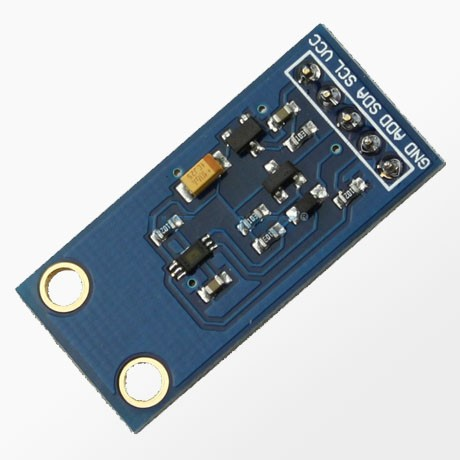
\includegraphics[width=0.4\linewidth]{Imagenes/gy-30}
\end{figure}

\subsubsection{Temperatura y Humedad DHT11}

``El DHT11 es un sensor de temperatura y humedad digital de bajo costo. Utiliza un sensor capacitivo de humedad y un termistor para medir el aire circundante, y muestra los datos mediante una señal digital en el pin de datos (no hay pines de entrada analógica). Es bastante simple de usar, pero requiere sincronización cuidadosa para tomar datos. El único inconveniente de este sensor es que sólo se puede obtener nuevos datos una vez cada 2 segundos, así que las lecturas que se pueden realizar serán mínimo cada 2 segundos''. \cite{DHT11}

\begin{figure}[H]
	\centering
	\caption[Sensor de temperatura y humedad DHT11.]{Sensor de temperatura y humedad DHT11. Tomado de: \cite{DHT11}}
	\label{fig:dht11}
	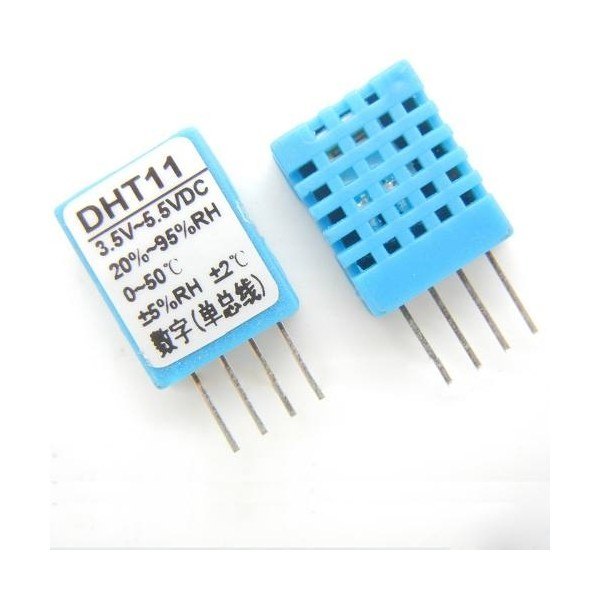
\includegraphics[width=0.4\linewidth]{Imagenes/dht11}
\end{figure}


\subsubsection{Módulo sensor de calidad de aire MQ-135}

La serie MQ de sensores de gas son sensores analógicos, por lo cual son fáciles de implementar con cualquier microcontrolador que posea un conversor analógico digital (ADC) adecuado. Estos detectores son electroquímicos y cambian su resistencia con la exposición a determinados gases, internamente poseen un calentador que se encarga de aumentar la temperatura interna para que el sensor pueda reaccionar con los gases provocando un cambio de valor en la resistencia, su estructura interior se puede observar en la Figura \ref{fig:estructura-del-sensor-mq}.\cite{MQ1}

\begin{figure}[H]
	\centering
	\caption[Estructura del sensor MQ.]{Estructura del sensor MQ. Tomado de: \cite{MQ1}}
	\label{fig:estructura-del-sensor-mq}
	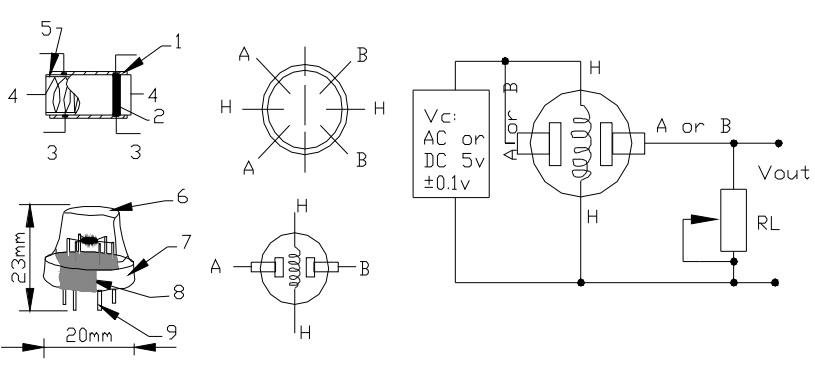
\includegraphics[width=0.7\linewidth]{Imagenes/Estructura_del_sensor_MQ}
\end{figure}

El Sensor Calidad Aire MQ135 se utilizan en equipos de control de calidad del aire a edificios y oficinas, son adecuados para la detección de NH3, NOx, alcohol, benceno, humo, CO2, etc; además de que estos sensores vienen en módulos como se observa en la Figura \ref{fig:sensor-calidad-aire-mq135}, lo que facilita su uso, simplemente se debe conectar al microcontrolador sin necesidad de utilizar algún circuito de acople. \cite{MQ1}

\begin{figure}[H]
	\centering
	\caption[Módulo sensor de calidad de Aire MQ-135.]{Módulo sensor de calidad de Aire MQ-135. Tomado de: \cite{MQ1}}
	\label{fig:sensor-calidad-aire-mq135}
 	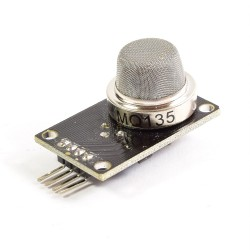
\includegraphics[width=0.35\linewidth]{Imagenes/sensor-calidad-aire-mq135}
\end{figure}

Este sensor es sensible en similar proporción a los gases mencionados, con lo que se puede determinar si el aire está limpio o si existe presencia de algún gas nocivo.\\

Los datos de salida de este sensor no son valores absolutos, simplemente proporciona una salida analógica que se debe monitorear y ser comparada con los valores típicos proporcionados en la hoja de datos.\cite{MQ2}

\subsubsection{Sensores de Estado}

Los sensores de estado describen si la variable está en alto (1) o en bajo (0), para estos detectores se tienen variables típicas, como el estado de una puerta o una ventana (abierta o cerrada), la lluvia, el movimiento.

\paragraph{Módulo detector de lluvia: }

Es un módulo relativamente simple que consiste en una serie de pistas conductoras organizadas de forma paralela e impresas sobre una placa de baquelita como se observa en la Figura \ref{fig:yl-83}. La separación entre sus caminos es muy pequeña, con el fin de crear un corto circuito cada vez que las pistas se mojan, ya que es un circuito abierto y el agua hace que se cree un camino de baja resistencia entre las pistas que tienen diferente potencial (Vcc-GND). La corriente que fluye a través de estas pistas se ve limitada por resistencias de 10K$\Omega$ en cada conductor, lo que impide que el corto circuito que se genera cuando se moja la placa vaya a estropear el micro controlador.\cite{LLU}

\begin{figure}[H]
	\centering
	\caption[Sensor de Lluvia.]{Sensor de Lluvia. Tomado de: \cite{LLU}}
	\label{fig:yl-83}
	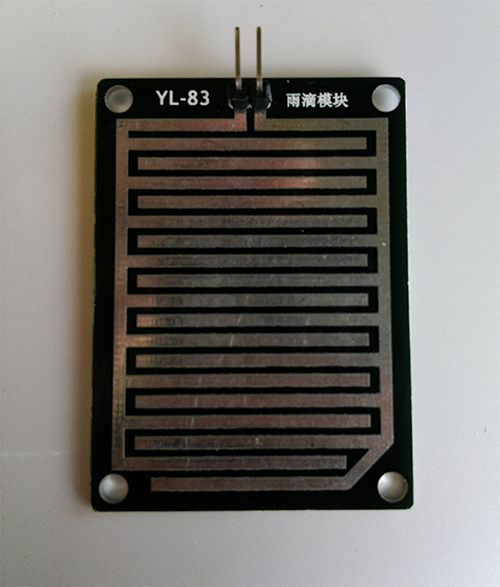
\includegraphics[width=0.35\linewidth]{Imagenes/YL-83}
\end{figure}

El circuito de control es el que posee las resistencias limitadoras de corriente y es el encargado de alimentar el módulo de la Figura \ref{fig:yl-83}. Como se observa en la Figura \ref{fig:yl-831} tiene un amplificador operacional, específicamente el circuito integrado LM392. Este se ocupa de amplificar el pequeño diferencial de voltaje que se produce cuando una gota de agua cae sobre las pistas del módulo. Aquí es donde se genera la señal de salida que puede ser del tipo analógica o digital. La señal digital oscilará entre los valores HIGH y LOW dependiendo de si hay agua o no sobre las pistas de la placa.\\

La salida analógica entregará un nivel de voltaje que variará dependiendo de la cantidad de agua que haya sobre el módulo.\cite{LLU}\\

\begin{figure}[H]
	\centering
	\caption[Módulo de sensor de lluvia.]{Módulo de sensor de lluvia. [Imagen Propia]}
	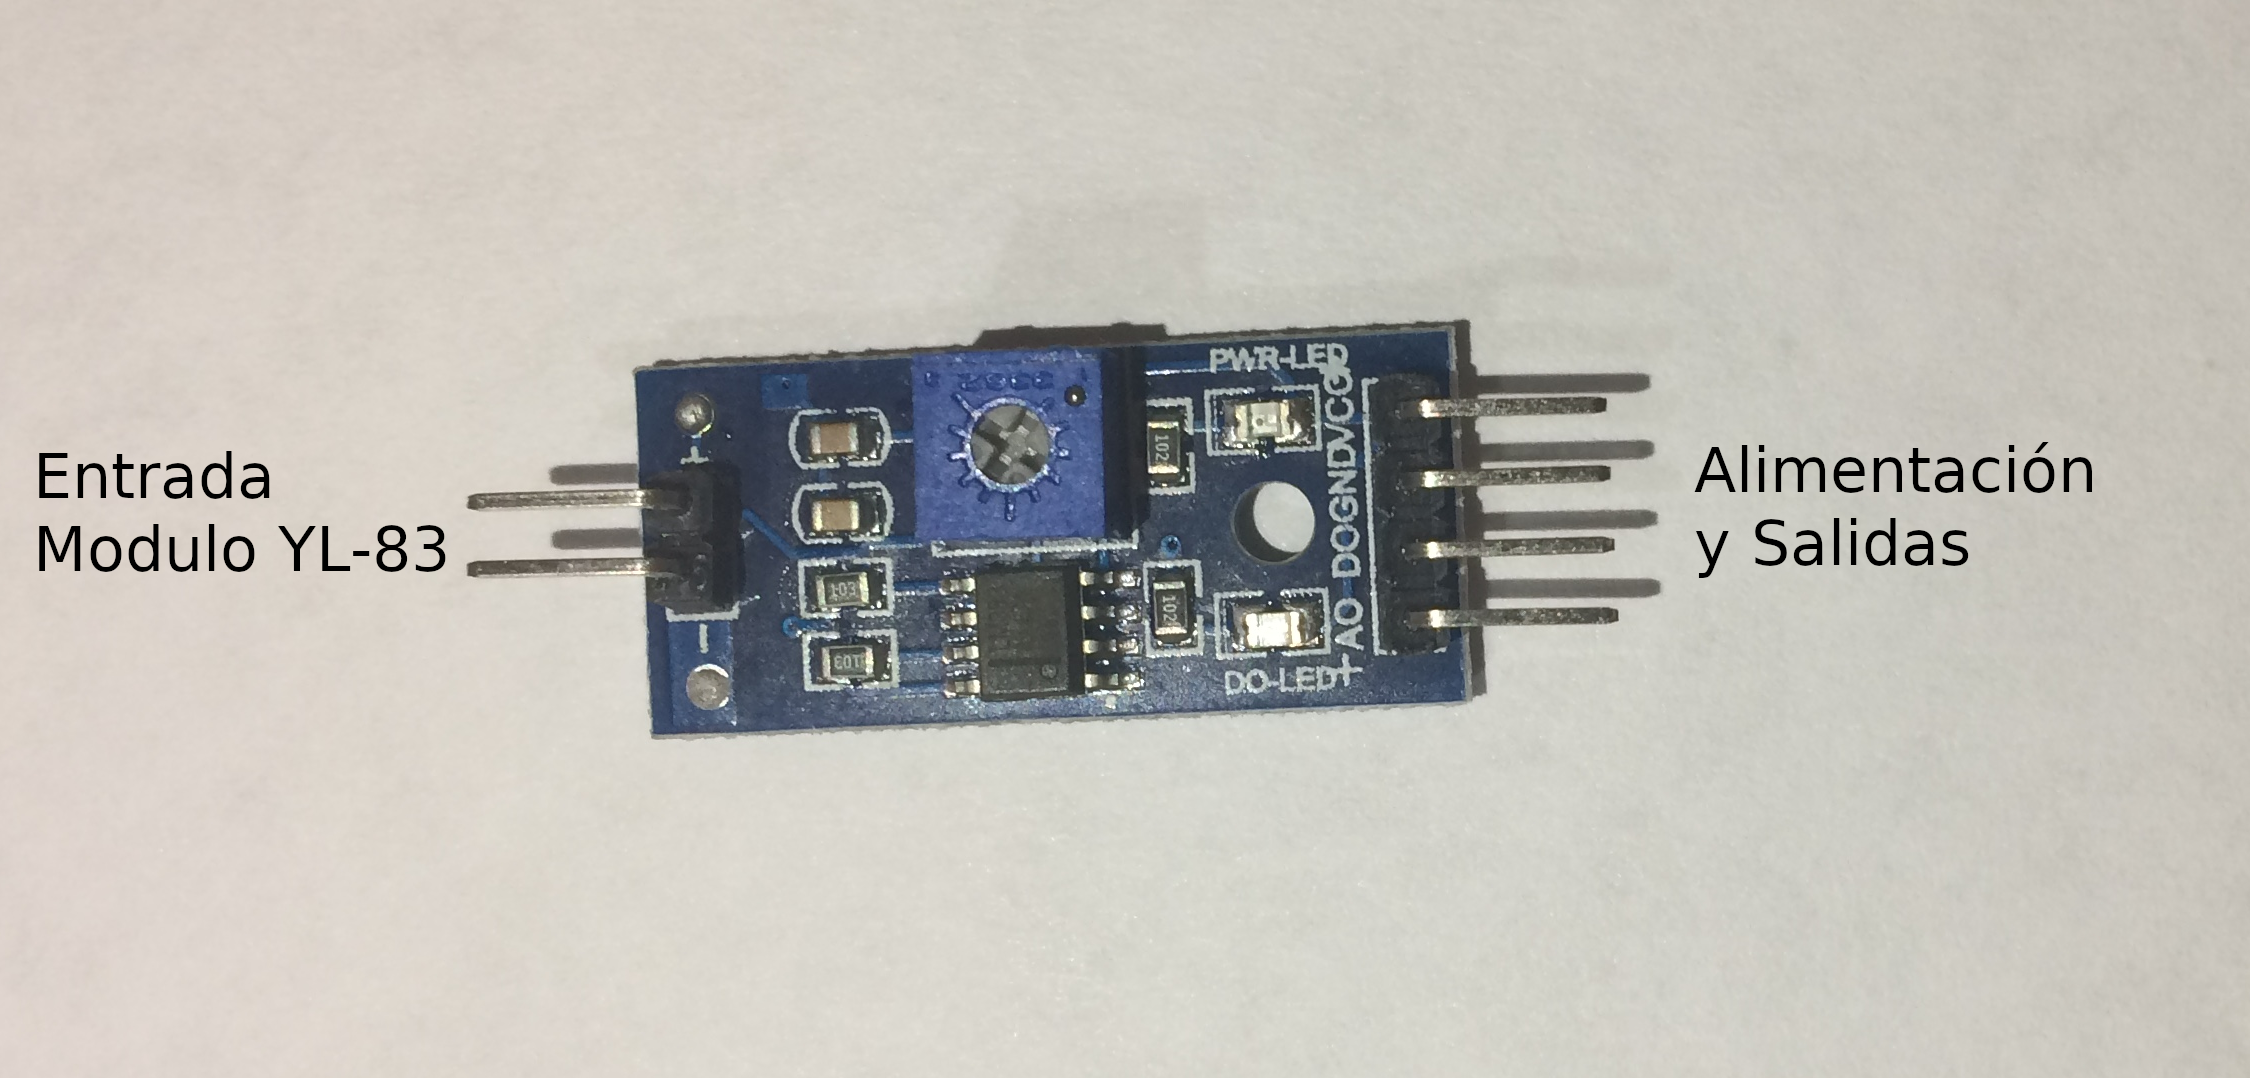
\includegraphics[width=0.5\linewidth]{Imagenes/YL-831}
	\label{fig:yl-831}
\end{figure}

\paragraph{Módulo PIR HC-SR501: }

La función de los sensores PIR es detectar movimiento, normalmente se busca detectar el movimiento de una persona dentro del rango del sensor. Son baratos, pequeños, de bajo consumo y fáciles de utilizar, además no se desgastan. Habitualmente se encuentran en electrodomésticos y gadgets para la oficina o el hogar. Son conocidos como PIR, ``Sensores Infrarrojos'' o ``Sensores de movimiento''.\\

Este módulo contiene un sensor Piroelectrico, el cual puede detectar niveles de radiación infrarroja como se observa en la Figura \ref{fig:sensor-hc-sr501-1000-m}. El detector de movimiento está dividido en dos mitades, la razón para esto es que se busca la diferencia en el movimiento y no el promedio. Las dos mitades están unidas de modo que se cancelan una a otra. Entonces, si una mitad recibe más o menos radiación IR, la salida cambiará a Alto o Bajo. \cite{PIR1}\\

El módulo PIR modelo HC-SR501, es pequeño y de bajo costo como se observa en la Figura \ref{fig:sensor-hc-sr501-1000-m}, incorpotando la tecnología más reciente en sensores infrarrojos pasivos para detectar movimiento. La emisión infrarroja se da en personas por su temperatura corporal y en animales (mamíferos), ya que emiten una radiación similar a los humanos. \cite{PIR2}

\begin{figure}[H]
	\centering
	\caption[Sensor HCSR501.]{Sensor HCSR501. Tomado de: \cite{PIR2}}
	\label{fig:sensor-hc-sr501-1000-m}
	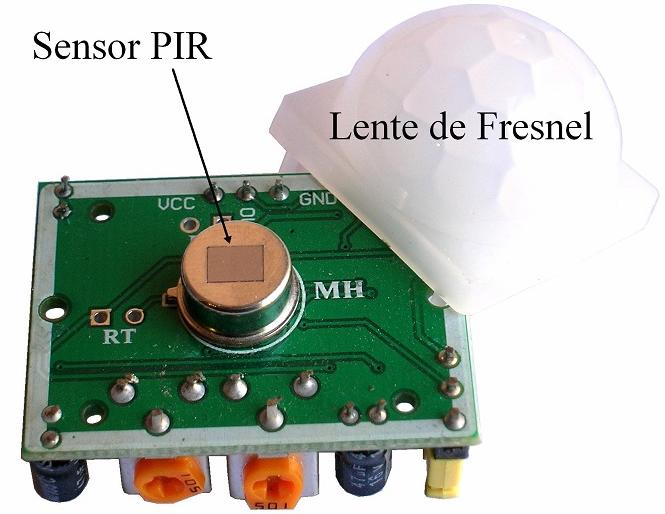
\includegraphics[width=0.5\linewidth]{Imagenes/SENSOR-HC-SR501-1000-M}
\end{figure}

\section{Software}

\subsection{RTOS}

Los sistemas operativos en tiempo real, tienen como parámetro clave al tiempo, ya que en gran variedad de situaciones, por ejemplo, un proceso industrial, se requiere recolectar múltiples datos, los cuales son usados para el control de diversos procesos que deben ser ejecutados en determinados instantes, de no ser así, podría causar desde la mala ejecución de una tarea, hasta un accidente según la delicadeza del proceso.\\ 

Para procesos con nula tolerancia a fallos, se conoce como un sistema en tiempo real duro, muchos de estos sistemas se encuentran en el control de procesos industriales, en aeronáutica, en la milicia y en áreas de aplicación similares. El caso contrario, cuando se tiene cierta permisividad a que muy ocasionalmente existan errores, se conoce como sistema en tiempo real suave, los sistemas de audio digital o de multimedia están en esta categoría. Los teléfonos digitales también son ejemplos de sistema en tiempo real suave. \cite{SO} \\

``Como en los sistemas en tiempo real es crucial cumplir con tiempos predeterminados para realizar una acción, algunas veces el sistema operativo es simplemente una biblioteca enlazada con los programas de aplicación, en donde todo está acoplado en forma estrecha y no hay protección entre cada una de las partes del sistema. Un ejemplo de este tipo de sistema en tiempo real es freeRTOS.  Las categorías de sistemas para computadoras de bolsillo, sistemas integrados y sistemas en tiempo real se traslapan en forma considerable. Casi todos ellos tienen por lo menos ciertos aspectos de tiempo real suave. Los sistemas integrados y de tiempo real sólo ejecutan software que colocan los diseñadores del sistema; los usuarios no pueden agregar su propio software, lo cual facilita la protección. \\

Los sistemas de computadoras de bolsillo y los sistemas integrados están diseñados para los consumidores, mientras que los sistemas en tiempo real son más adecuados para el uso industrial. Sin embargo, tienen ciertas características en común''. \cite{SO}

\subsection{ESP-IDF}

ESP-IDF es el entorno de desarrollo oficial para el ESP32 desarrollado por Espressif System, el cual mediante una serie de comandos específicos escritos en la terminal (en el caso de linux), habilita la configuración del ESP32 en cuanto a su funcionamiento, es decir, permite encender o apagar características como el WiFi, el Bluetooth o realizar particiones de memoria, además de esto, se puede cargar el código por el puerto USB al ESP32, al igual que visualizar la información generada por el ESP32 por el mismo puerto. Este entorno se encuentra construido con diferentes características y APIs, algunas de ellas se mencionan a continuación. \cite{ES}

\paragraph{FreeRTOS:}el framework está desarrollado sobre este sistema operativo de tiempo real, tomando algunas funcionalidades propias, como la tareas y las colas.

\paragraph{Wi-Fi:}el módulo ESP-WROOM-32 posee la capacidad en el hardware para la conexión a una red Wi-Fi, y este software proporciona las librerias y las funcionalidades a fin de realizar dicha conexion y enviar o recibir datos.

\paragraph{Particiones:}el MCU contiene una memoria flash, la cual por medio de este framework se le pueden realizar particiones, dedicadas a almacenar la lista de instrucciones, y también para guardar ciertos archivos. Estas se configuran a través de un fichero csv.

%\paragraph{Consola:}el framework provee una libreria para realizar la programacion de una consola, con el fin de ejecutar diferentes funcionalidades programadas dentro del sistema por el desarrollador.

\paragraph{HTTP Request:}para realizar diferentes peticiones HTTP como las descritas anteriormente, el entorno de desarrollo cuenta con la librería LWIP encargada de realizarlas.

\paragraph{Timers:}este framework provee varias funciones con el objetivo de disponer de los timers de 64 bits que posee el ESP32 y además para configurar sea un timer periódico o de un solo disparo.

\subsection{Proteus}

Proteus combina facilidad de uso con características de gran alcance con la finalidad de ayudar a diseñar, probar y concebir PCB profesionales. Con casi 800 variantes de microcontroladores listos para la simulación directamente desde el esquematico. Además de contar con uno de los paquetes de diseño de PCB profesionales más intuitivas en el mercado y un autoruteo de clase mundial incluido como estándar. \cite{Prot1} \\

Además, es una herramienta muy completa y potente de simulación de circuitos y diseño de PCBs. Dentro de la simulación de circuitos admite componentes pasivos, digitales, analógicos y componentes más complejos como LCDs y motores. Por tanto, se puede realizar casi cualquier cosa, el programa está pensado para que una vez se tenga el circuito diseñado se pueda pasar a una PCB \cite{Prot2}. Adicionalmente los dispositivos que no se encuentren se pueden agregar, ya sea de la página oficial o construyéndolos en el software por medio de las funcionalidades provistas.
